\chapter{Methods}\label{chapter:methods}
In order to accurately determine the characteristic parameters of a VECSEL chip, it is necessary to have an experimental setup that can measure a small change, in the order of \qty{0.1}{\percent} in the reflectivity over a dynamic range of about 4 order of magnitude in pulse fluence. A dedicated setup fulfilling these criteria has been constructed and utilized by  (INSERT HERE REFERENCES).

For the measurements, a total of 4 different VECSEL chip were used, with three of them having a different structure (further discussed in \cref{sec:vecsel}). We were interested on the impact of different pump powers and the temperatures on the characteristic parameters of the VECSEL across the three different structures. For this we measured the nonlinear reflectivity for each chip for 9 different pump powers in the range from \qtyrange{0}{16}{\watt} and for three temperatures \qtylist{-10;0;10}{\degreeCelsius}.

The subsequent section provide an overview of the different VECSEL structures, the measurement setup and the data processing method.

\section{VECSEL Chips}\label{sec:vecsel}

TODO: redo design images maybe with legend? different colors?

The basic structure of a VECSEl gain chip is shown in \cref{fig:vecDes}. The main feature of the structure are as follows: 

\begin{itemize}
    \item Heat spreader: The heat spreader role is in dissipating the heat generated during the operation of the VECSEL chip to a Peltier-controlled copper heat-sink.
    \item Pump \& laser  DBR: The purpose of the two bottom mirrors is to reflect the laser light and the pump light. There are two main advantages to this approach: firstly, because of higher absorption, there is a higher optical-to-optical efficiency due to the two passes through the active region, and secondly, there is less absorption in the mirror and in the heat sink, which results also in a higher efficiency and a higher maximum output power. The high reflectivity for two wavelengths is realized by using a distributed Bragg reflector (DBR)
    \item Active region: The purpose of the active region is the conversion of the pump light into the laser light. The gain medium in the active region is often composed of quantum wells or quantum dots.
    \item Anti-reflection coating: The antireflection section is optimized to reduce the otherwise large reflection from the air/GaAs interface
\end{itemize}

Below the three different structure of the Vecsel chips used in this work.

\begin{figure}[ht]
    \centering
    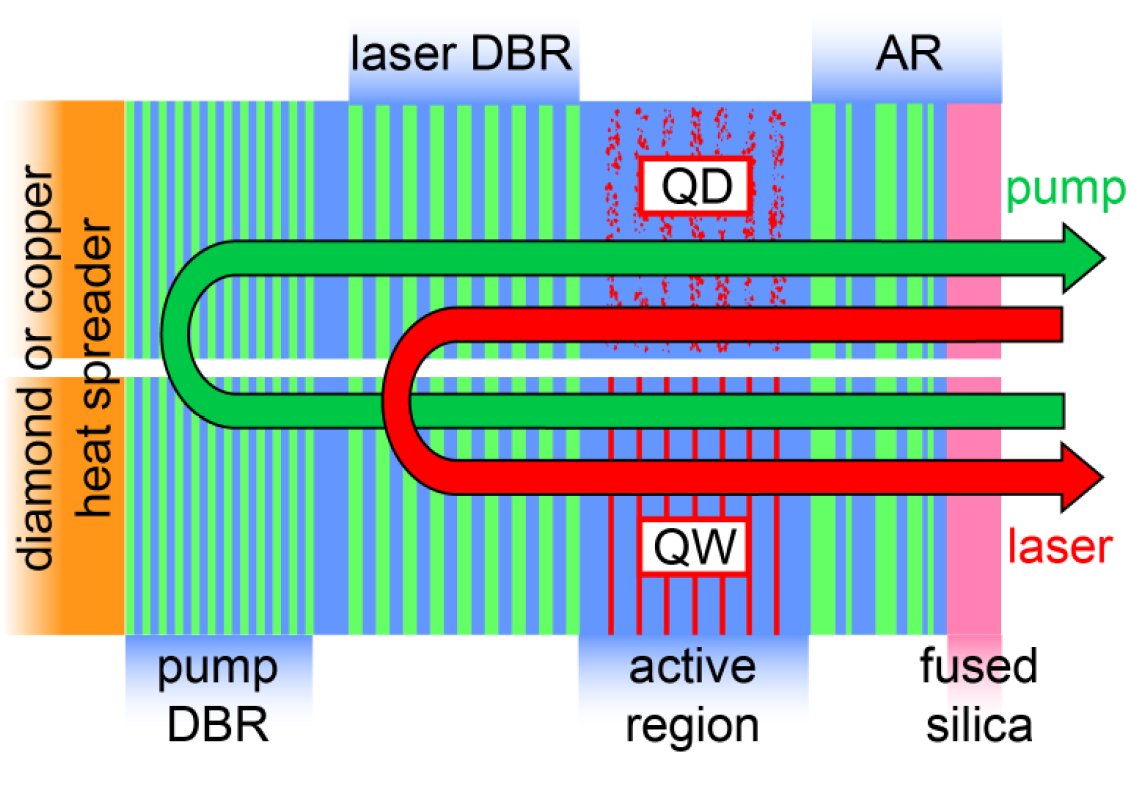
\includegraphics[width=.6\linewidth]{images/VECSEL_structure.png}
    \caption{TODO: caption}
    \label{fig:vecDes}
\end{figure}


%A distributed Bragg reflector (DBR) for the pump wavelength (808 nm) reflects the unabsorbed pump light, reducing heat deposition in the structure and increasing efficiency.
% The DBR for the laser wavelength acts as a flat cavity mirror.


\subsection*{No pump DBR chip, SV166}

\begin{wrapfigure}{r}{.4\textwidth}
    \vspace{-\baselineskip}
    \centering
    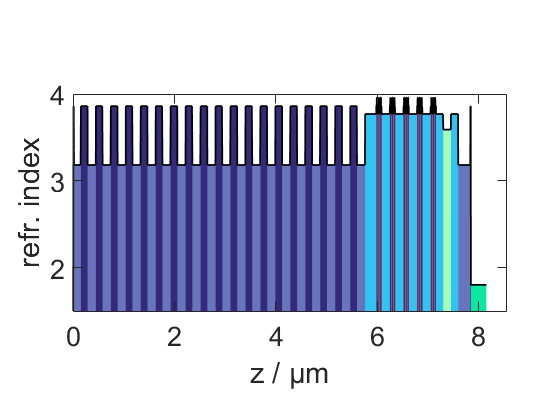
\includegraphics[width=.98\textwidth]{images/1SV166.lay.png}
    \caption{TODO: caption}
    \label{fig:sv166}
\end{wrapfigure}

This structure has an antiresonant design and cooled from the backside by a copper heat spreader. The DBR consists of 19-pairs of GaSb/AlAs\textsubscript{0.08}Sb\textsubscript{0.92} layers design around a wavelength of \qty{2080}{nm}. The active region has $5\times3$ In\textsubscript{0.27}Ga\textsubscript{0.73}Sb quantum wells (QW) placed at the maximum of the standing-wave cavity. Additional barriers layer made of AlAs\textsubscript{0.08}Sb\textsubscript{0.92} are placed around the gain QW to increase the photoluminesence. The last layer is a PECVD coating made of Si\textsubscript{3}N\textsubscript{4}, which serves an an antireflection coating.


\subsection*{Pump DBR chip, SV167}

\begin{wrapfigure}{r}{.4\textwidth}
    \vspace{-\baselineskip}
    \centering
    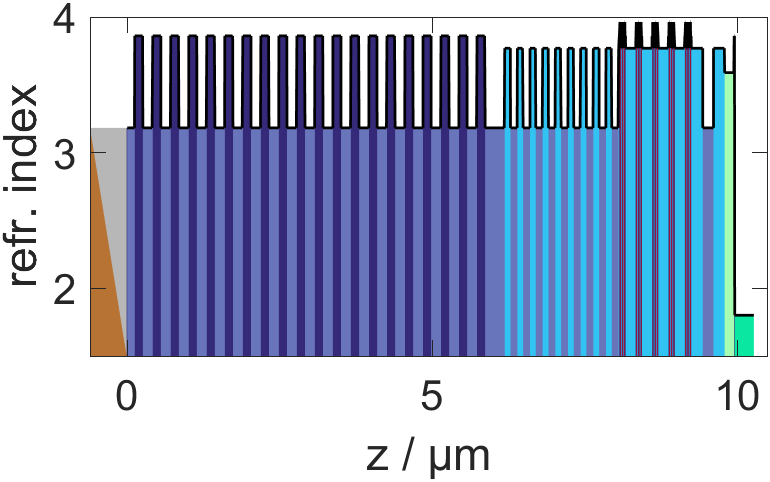
\includegraphics[width=.98\textwidth]{images/1SV167B.lay.png}
    \caption{TODO: caption}
    \label{fig:sv167}
\end{wrapfigure}

This is a similar strucutre as above but this time including an extra DBR for the pump wavelength of \qty{1470}{\nm}. The pump DBR is made of 10 layers of Al\textsubscript{0.2}As\textsubscript{0.8}Sb/Al\textsubscript{0.15}Ga\textsubscript{0.85}AsSb. For the thickness of the layers the \qty{45}{\degree} incident of the pump beam had to be accounted for. This strucutre was measured twice but for different heat spreaders, one made of copper and the other of diamond, to observe and compare the influence of better thermal conductovity of the heatsinks.


\subsection*{Hybrid chip, SV165}

\begin{wrapfigure}{r}{.4\textwidth}
    \vspace{-\baselineskip}
    \centering
    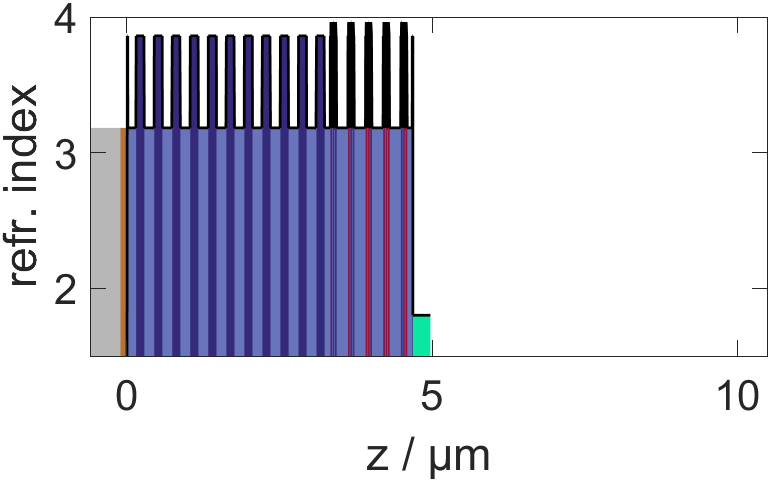
\includegraphics[width=.98\textwidth]{images/1SV165.lay.png}
    \caption{TODO: caption}
    \label{fig:sv165}
\end{wrapfigure}

This sturcutre incorbareted a hybrid metal-semiconductor Bragg reflector. It consisted of a  \qty{100}{\nm} copper layer with 10.5 AlAs\textsubscript{0.08}Sb\textsubscript{0.92}/GaSb layers. This allows for a thinner gain chip design of just under \qty{5}{\um} compared to the other strucutres \qty{7.5}{\um} resp. \qty{10}{\um} for the pump DBR design. This lowered the thermal resistance of the device by \qty{24}{\percent}. This structure also has a different active region made of $5\times3$ In\textsubscript{0.27}Ga\textsubscript{0.73}Sb/GaSb QW.

\section{Experimental setup}\label{sec:setup}

The experimental setup is depicted in \cref{fig:setup}. The setup is driven by a modelocked Ti:sapphire laser. The laser emits femtosecond pulses at a wavelength of \qty{810}{\nm}, with a repletion rate of \qty{80}{\MHz} and an average output power of \qty{4}{\W}. The laser beam then passes through an optical parametric oscillator (OPO), where the beam undergoes nonlinear frequency conversion resulting in two waves: an idler wave and a signal wave. The OPO idler wave can be tuned from \qtyrange{1.7}{4}{\um} and has a maximum output power of \qty{650}{\mW}. The idler has been tuned to a specific wavelength of \qty{2071.7}{\nm} and was stabilized using an integrated automated feedback loop.

To further achieve a wide range of pulse fluences, the laser beam is directed through two wire-grid polarizers. One of the polarizers is placed on a controllable rotation stage to adjust the beam attenuation. The wire-grid polarizers have a broad range of attenuation across different wavelengths and do not alter the beam path during rotation. After the attenuation stage, the beam passes through a beamsplitter, which separates it into two arms: the reference arm and the sample arm. 

The reference arm contains a high-reflection mirror of known reflectivity from which the leaking signal is collect in a photo diode to monitor the fluence during a measurement. 
The VECSEl chip is placed at the end of the sampel arm. Before the beam is incident on the VECSEL, a focusing lens is used to achieve higher fluences on the VECSEL. The VECSEL is probed under a direct incidence angle, and its reflection is collected using the same lens. Both beams are recombined at the beamsplitter and direct to an integrating sphere photodiode to measure the total reflected power. The pump beam enters from the side at a \qty{30}{\degree} angle and is shown in green. 

To measure the different signals from the two different arms and also measure the photoluminescence (PL) signal of the pumped VECSEL chips, two choppers are used. The two choppers separte the signals in time allowing to measure the signals with the same detector. The choppers are phase locked and chopper 2 is run at half of the frequency of chopper 1, specifically at \qty{55}{\Hz}. Chopper 2 is placed in the beam path before the attenuator to block the beam during every second cycle of chopper 1. This allows to isolate the PL signal. Chopper 1 is placed such that both arms can be intercepted by the blades, enabling the passage of light from both or either of the arms. During one cycle of chopper 2, five distincte state can occur, each allowing for a different measurement configuration:
\begin{enumerate}
    \item Only the sample signal, composed of the photoluminescence and the sample signal (S+PL)
    \item Both arms are open, allowing the compined singal from the sample and reference arm  (S+PL+M)
    \item Only the reference signal (M)
    \item Both arms are blocked and only the background signal from the detector is measured (Z)
    \item The probe beam gets blocked and only the (PL) signal is measured
\end{enumerate}

To obtain the reflectivity from the VECSEL, the (PL) and the background signal (Z) are substracted from the sample signal (S+PL). The resulting value is then compared the reference measurement (M). This yields a scaling factor R, which then can be used to calculate the reflectivity based on the known reflectivity of the reference mirror. To obtain accurate measurement point, 200 such signal iteration are averaged together for the final measurement point.
\newpage

\begin{figure}[ht]
    \centering
    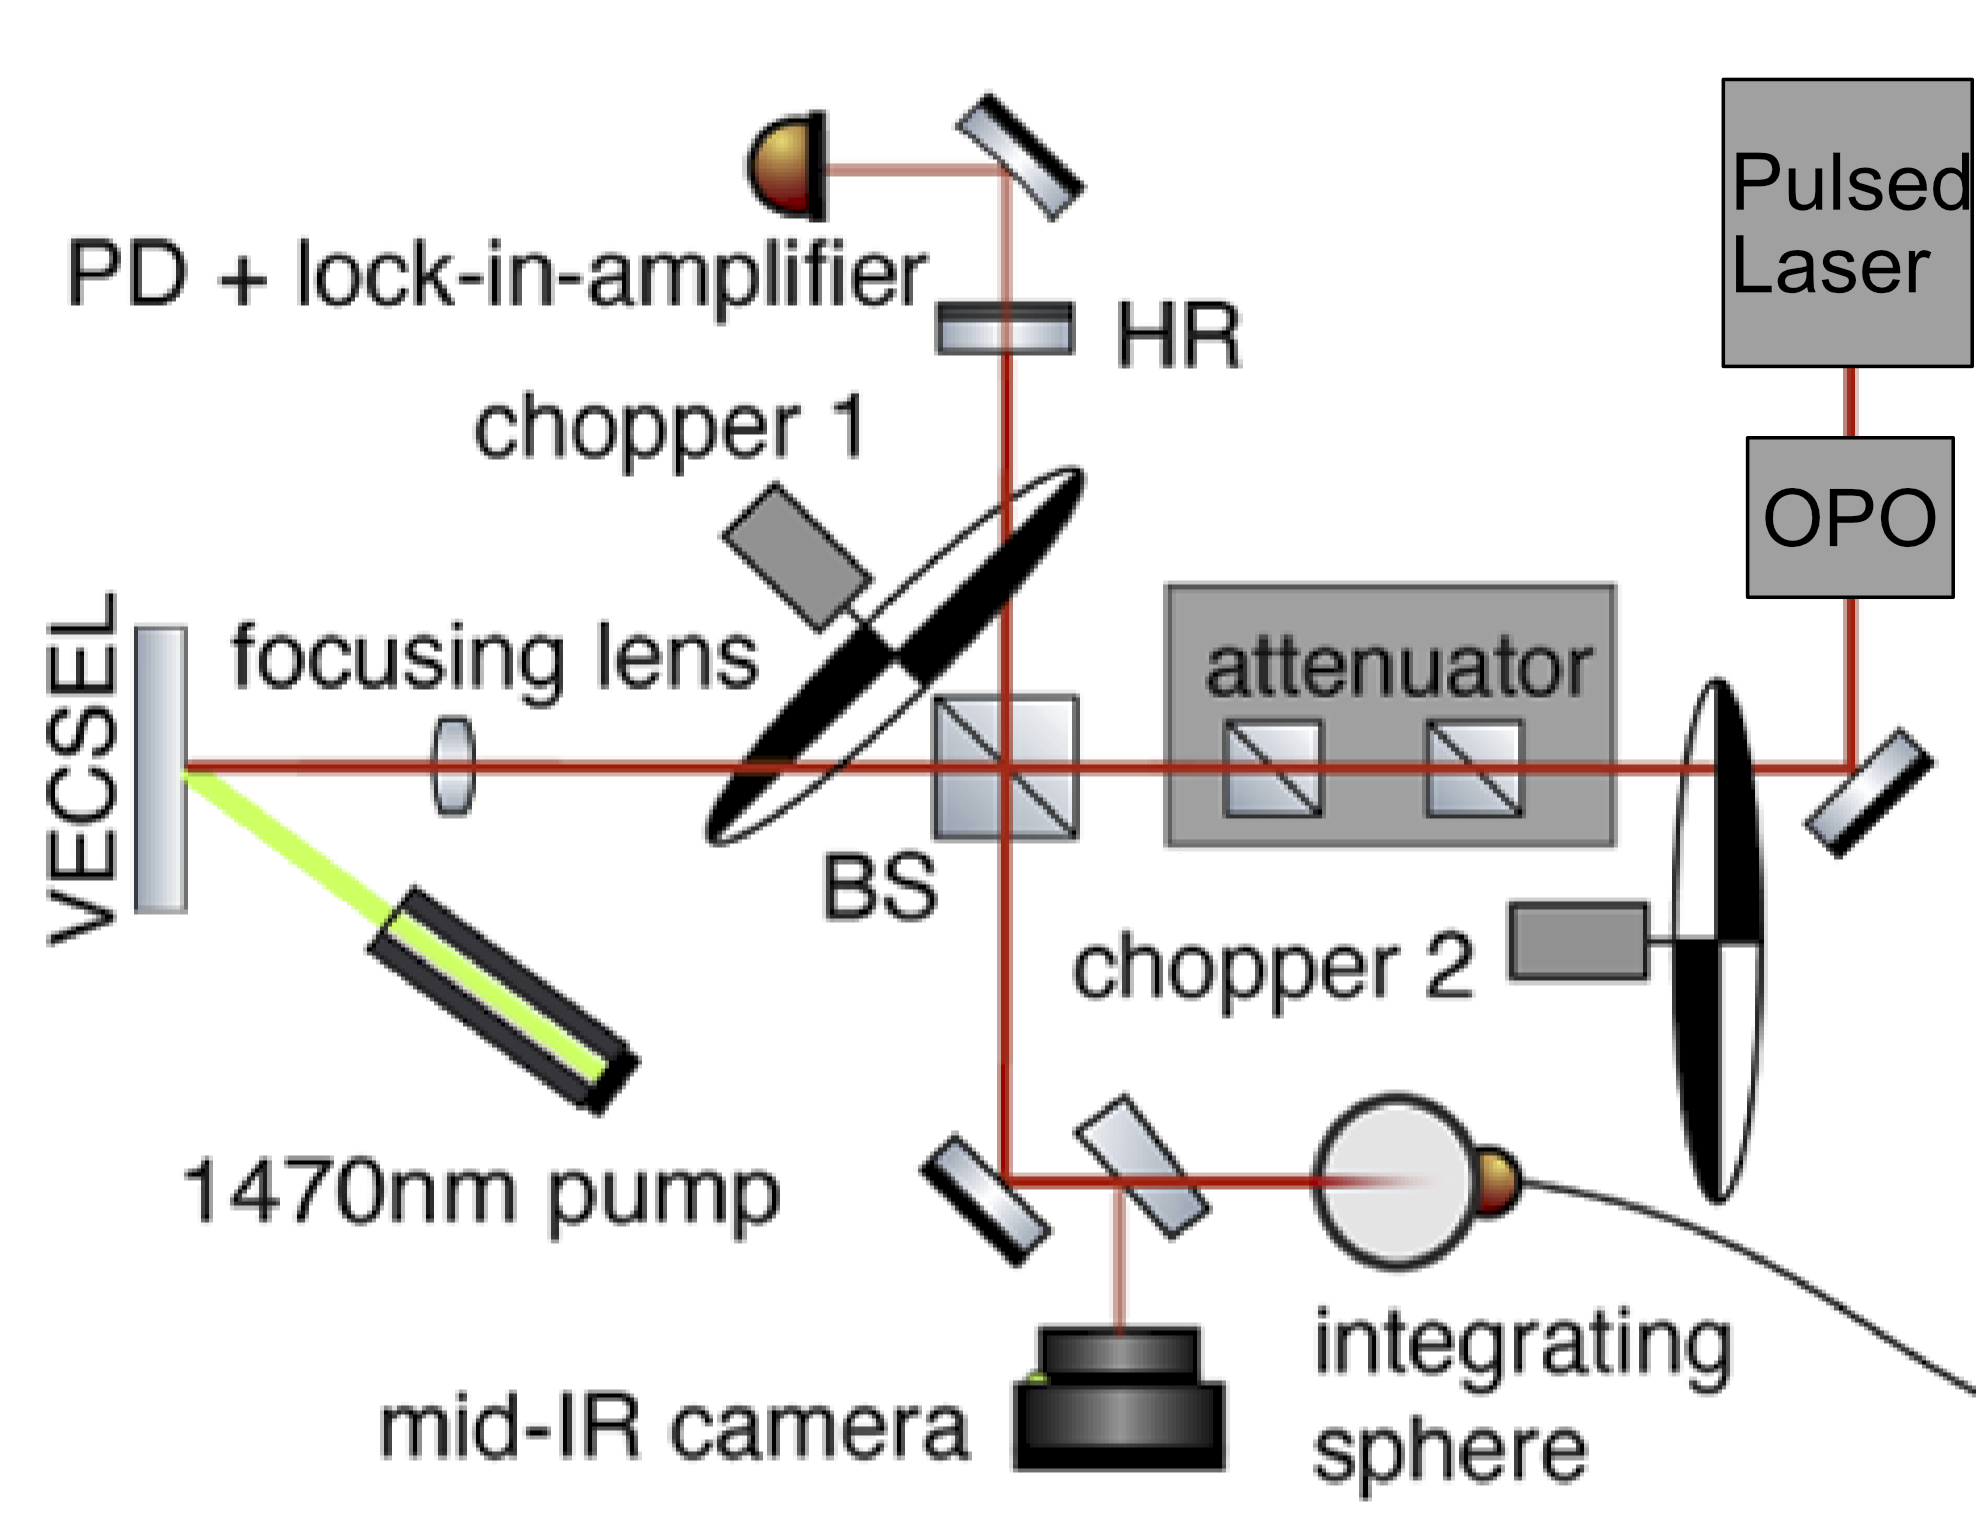
\includegraphics[width=0.8\linewidth]{images/setup.png}
    \caption{On top: Experimental Setup for gain characterization of VECSEL chips. The laser source is a tunable optical parametric oscillator pumped by a modelocked Ti:sapphire laser. An attenuation stage controls the incidient probe fluence on the VECSEL. The pump beam enters the setup at a \qty{30}{\degree} angle. Two choppers, phase-locked and operating at different frequencies, are positioned to differentiate signals and measure photoluminescence (PL) emitted by the pumped VECSEL chip. The figure showcases the key components and their relative positions within the experimental setup.
    On bottom: Visualization of the five different configuration of the two choppers and the measured signal, adjusted from REFERENCE.}
    \label{fig:setup}
\end{figure}

\subsection{Automation of the pump power}{\label{subsubsection:pump}}

To improve the time efficiency and increase the unattented measuring time of the experimental setup, the control of the pump power has been automated. In the original setup, the pump power of the laser diode was controlled over a Delta Elektronika SM 18-50 DC power supply, which can deliver up to \qty{50}{\ampere} at up to \qty{18}{\volt}. The power supply was connected over a serial interface controller to a computer and be integrated into the already existing user interface of the measurement setup. To implement the control of the pump, a new text field has been added to the user interafce where a list of current values for the power supply can be added. Instead of specifiying power values directly, the decisionaws made to enter current values instead due to the ptoential for exchaning the pump laser diode in the future, which would necessitate to adjust the controller in the software. The software then iterates over this lists and makes a complete measurement for each current value in the list. However, the full automation also required to adjust the signal processing algorithm of the software, which will be discussed in the next section. 

\begin{figure}[ht]
    \centering
    \sidesubfloat[]{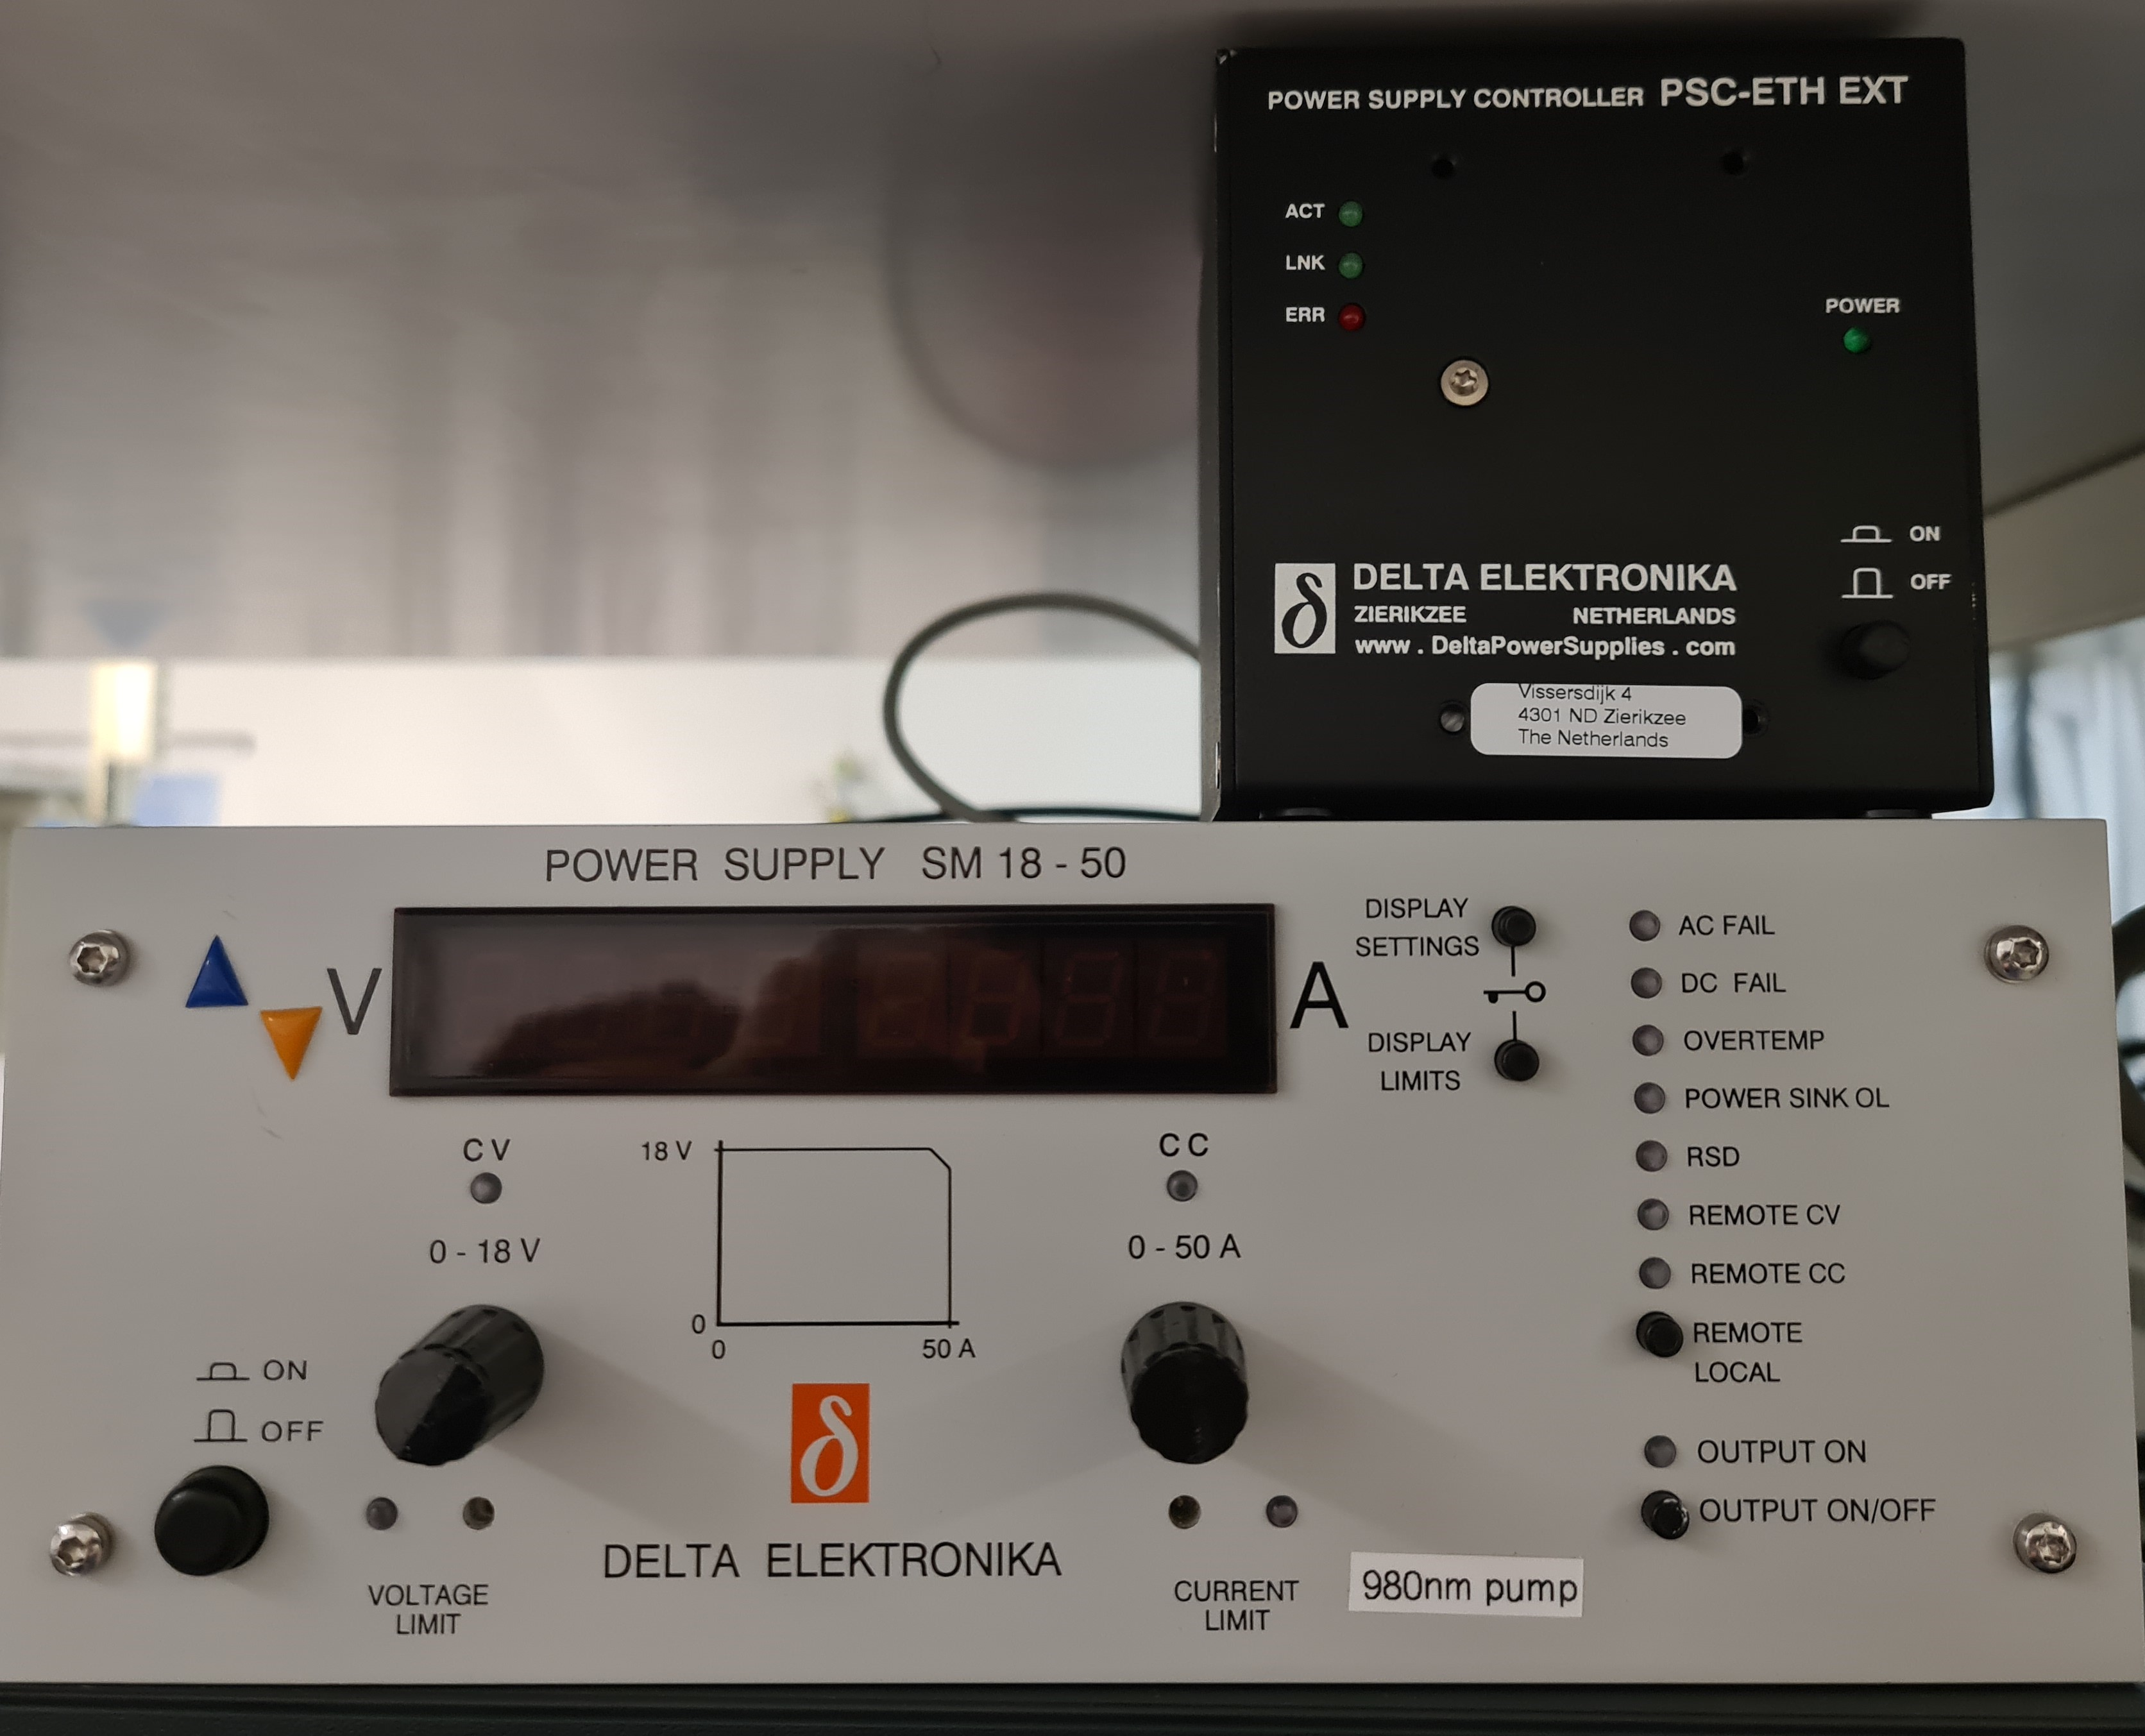
\includegraphics[height=4.5cm]{images/powersupply.jpg}\label{fig:supply}}
    \hfill
    \sidesubfloat[]{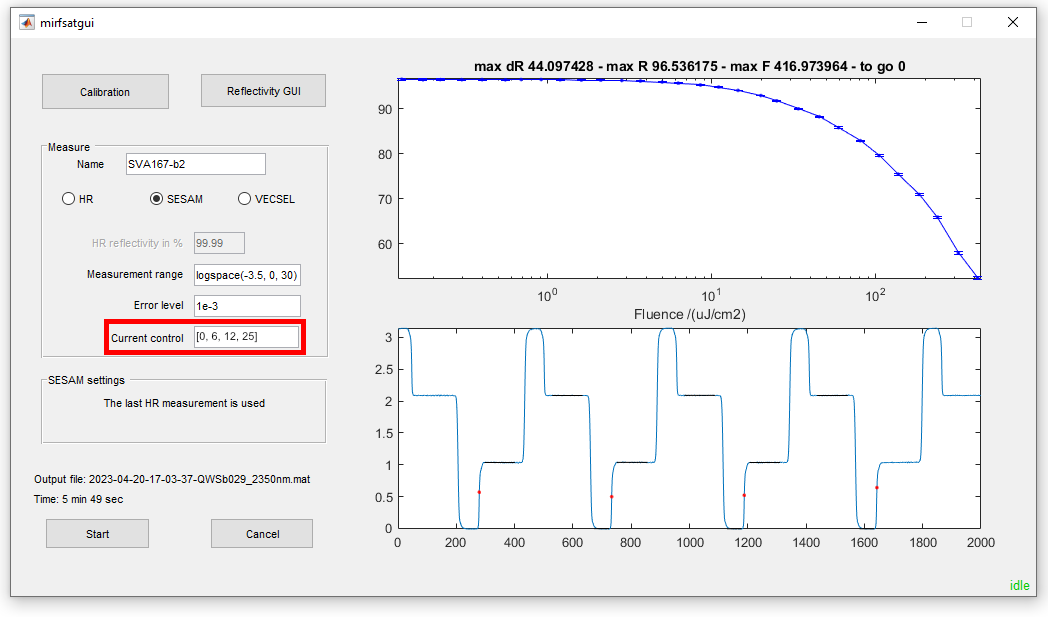
\includegraphics[height=4.5cm]{images/software.png}\label{fig:software}}
    \caption{TODO: ADJUST SOFTWARE PICTURE AND WRITE CAPTION}
    \label{fig:auto}
\end{figure}


\section{Data processing}\label{sec:processing}

The PD signal is amplified by a computer-controlled variable pre-amplifier to use the full
range of the AD converter. The absolute gain and the offset have no influence on the
measurement accuracy, it is only necessary to provide a linear response. Since the reflectivity
R is encoded in only one optical/electrical signal the constraints on the amplifier have become
negligible. This is in contrast to the method of Haiml et al., in which the same gain and no
offset has to be achieved by both amplifiers [16].
The computer algorithm first detects the rising edges (red dots in Fig. 4(c)) and then takes
the mean value of the data points on the flat levels (red lines in Fig. 4(b)). As both beams are
blocked in phase 4, we can precisely measure the offset of the photodiode. Level A and B
(Fig. 4(b)) are obtained by subtracting the signal level in state 1, and the nonlinear reflectivity
is obtained as R = B / A. This is done for 500 periods in succession (takes approximately 5
seconds per fluence) and averaged to minimize detector noise and laser noise. This averaged
reflectivity has a standard deviation of 0.01\%. The incident fluence can be computed from the
level A and the pre-amplifier gain setting. An accuracy of 5\% for the fluence measurement is
typically good enough, as this will afterwards result in an inaccuracy of 5\% for the fitted
saturation fluence Fsat.

\begin{figure}[ht]
    \centering
    \sidesubfloat[]{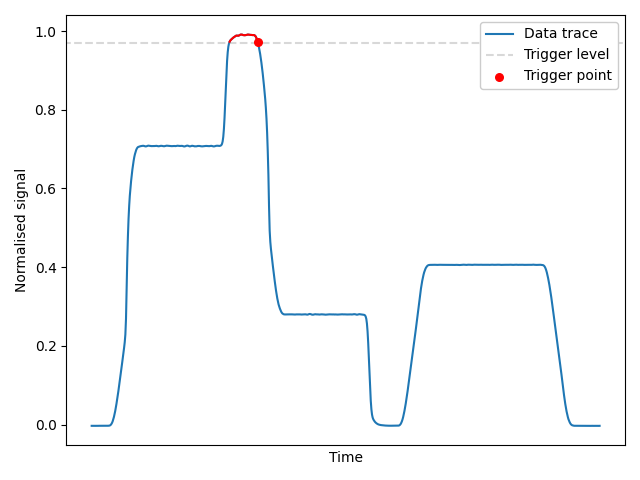
\includegraphics[width=0.29\linewidth]{images/old_trace.png}\label{fig:a}}
    \sidesubfloat[]{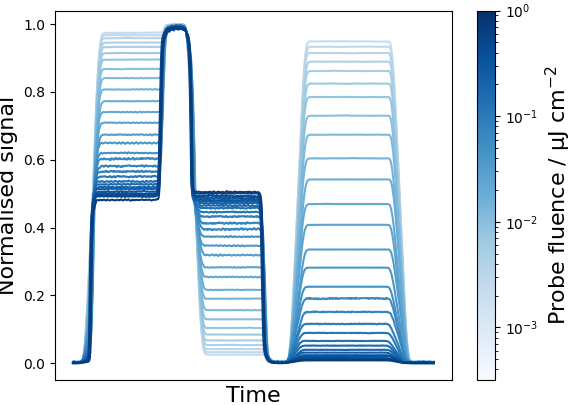
\includegraphics[width=0.29\linewidth]{images/trace_complete.png}\label{fig:b}}
    \sidesubfloat[]{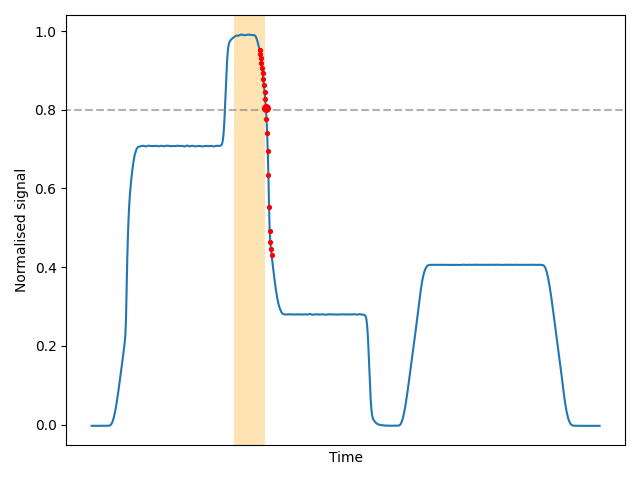
\includegraphics[width=0.29\linewidth]{images/corrected_signal.png}\label{fig:c}}
    \caption{Main caption}
\end{figure}


